% Anonymised manuscript for double-blind review (Journal of Geographical Systems).
% Compiles with pdflatex + bibtex. To move to the Springer Nature template, replace the preamble with
%   \documentclass[pdflatex,sn-basic]{sn-jnl}
% and keep the body unchanged (author-year citations via natbib are supported by sn-basic).
\documentclass[11pt]{article}
\usepackage[T1]{fontenc}
\usepackage[utf8]{inputenc}
\usepackage{mathptmx}
\usepackage[a4paper,margin=2.5cm]{geometry}
\usepackage{setspace}\doublespacing
\usepackage{lineno}\linenumbers
\usepackage{amsmath,amssymb,bm}
\usepackage{graphicx,booktabs,multirow,array,threeparttable}
\usepackage[labelfont=bf,labelsep=space,font=small]{caption}
\DeclareCaptionLabelFormat{figfmt}{Fig.~#2}
\captionsetup[figure]{labelformat=figfmt}
\usepackage{placeins}
\usepackage{rotating}
\usepackage{tikz}\usetikzlibrary{positioning,arrows.meta,fit,calc}
\usepackage[authoryear,round]{natbib}
\usepackage[hidelinks]{hyperref}
\usepackage{xurl}
\setcitestyle{aysep={}}
\newcommand{\HMX}{HiST-MAT-X}

\title{When does cross-city transfer help? A three-city benchmark for incident-level crime prediction under short local histories}
\date{}

\begin{document}
\maketitle
\vspace{-3em}

\begin{abstract}
\noindent Law enforcement agencies regularly lose usable crime histories when record systems, geographic units or reporting standards change, yet models that infer an incident's crime type or time of day are trained on years of local data. We ask whether models trained in other cities can stand in for missing local history. Using 4.8 million harmonised incidents from Chicago, New York and San Francisco (2019--2026), we build a benchmark where a target city receives 0, 4, 8, 16 or 52 weeks or its full history, all methods share the same 26 test weeks, and inference uses a week-block bootstrap. We compare 12 models, including pooled gradient boosting, a tabular foundation model, a source-pretrained FT-Transformer and \HMX{}, a masked multi-attribute transformer on city-agnostic history features. With four weeks of history, the two source-pretrained models beat the best target-only model in 23 of 24 model--city--task comparisons over two test windows in opposite seasons, by up to 0.037 nats. At eight weeks the benefit was smaller and season-dependent, and by 16 weeks it had vanished. Gains were largest in low-volume areas and clustered in space only as far as volume did. Pooling raw incidents was no reliable substitute. \HMX{} matched or slightly trailed the task-specific pretrained FT-Transformer while training one model for both tasks 4.8 to 9.3 times faster, and its zero-shot predictions matched or beat four weeks of local data in three of six cases per window. Cross-city pretraining is thus a short-term bridge, not a replacement for local data.
\end{abstract}

\noindent\textbf{Keywords} Crime prediction $\cdot$ Transfer learning $\cdot$ Spatio-temporal heterogeneity $\cdot$ Short histories $\cdot$ Tabular deep learning $\cdot$ Spatial autocorrelation

\noindent\textbf{JEL Classification} C45 $\cdot$ C53 $\cdot$ K42 $\cdot$ R19

% ======================================================================
\section{Introduction}\label{sec:intro}

Crime is concentrated in a small share of places and recurs there over time \citep{weisburd2015}. Much of the predictive value of police records therefore lies in local history: the recent mix of offences in a neighbourhood, the hours at which incidents cluster, and how these change from week to week. Statistical and machine-learning models that exploit this regularity range from self-exciting point processes \citep{mohler2011} to deep spatio-temporal networks for region-level forecasting \citep{huang2018deepcrime,xia2021stshn,li2022sthsl} and short-term hotspot prediction from dynamic urban features \citep{rumi2018}. A systematic review lists open police data from large US cities, Chicago and New York among them, as common data sources in this literature \citep{mandalapu2023}.

All of these approaches assume that a long, consistent local history is available. In practice that assumption often fails. Agencies migrate record-management systems, adopt new offence taxonomies, redraw reporting areas or publish open data for the first time. Each change leaves the agency, or an analyst working with its data, with weeks rather than years of comparable records. The question we study is whether models trained in other cities can fill this gap, and if so, for how long.

Cross-city transfer is well studied for urban flows such as traffic and bike demand \citep{wang2019regiontrans,yao2019metast,jin2022crosstres}. For crime, transfer has been explored mainly for counts or occurrence on grids and regions \citep{zhao2017transfer,bappee2021,wu2024transfer,karimova2025,shan2026}, with the most recent work relating transfer performance to differences between cities \citep{shan2026}. Cities also differ in how strongly crime clusters in space \citep{walter2023}, which makes it unclear how much transferable structure exists. Incident-level tasks, such as estimating the offence type of an incident from where and when it was reported or estimating the time of day from where it happened and what it was, have to our knowledge not been studied under transfer at all, even though they underpin data-quality checks, imputation of missing fields and resource planning.

Recent progress in tabular deep learning makes the question timely. Pretrained tabular foundation models make strong predictions from small training sets \citep{hollmann2025,qu2025tabicl}. Deep tabular models have caught up with gradient boosting when given enough tuning and ensembling \citep{gorishniy2025,erickson2025}, although tree ensembles long dominated and remain strong \citep{grinsztajn2022,erickson2025}. Supervised pretraining on related tables transfers well, especially when downstream data are scarce \citep{levin2023}. None of these results has been tested on crime records, where label distributions shift between cities and the same feature can mean different things in different places.

This paper makes four contributions.
\begin{enumerate}
\item \textbf{A cross-city short-history benchmark} for incident-level crime type (10 harmonised types in 3 groups) and time-of-day (6 slots) prediction in Chicago, New York and San Francisco. Target cities receive 0, 4, 8, 16 or 52 weeks or their full history, all methods share the same 26 test weeks, history features are computed online, and inference uses a week-block bootstrap.
\item \textbf{An answer to when pretraining helps.} With four weeks of history, source pretraining improves on the best target-only model in every city and task, and this replicates on a second test window in the opposite season. At eight weeks the benefit is smaller and season-dependent, and by 16 weeks it has disappeared in both windows. Pooling raw incidents from other cities into gradient boosting is not a reliable substitute. The gains are largest in low-volume areas, and their spatial clustering is fully accounted for by the clustering of area volume.
\item \textbf{\HMX{}}, a masked multi-attribute transformer whose inputs are city-agnostic summaries of recent local crime, with a coherent hierarchy loss over the offence taxonomy. One model serves both tasks and supports zero-shot prediction. It matches or slightly trails a task-specific pretrained FT-Transformer while training 4.8 to 9.3 times faster.
\item \textbf{A transparent account of what does not work}, including pre-specified hypotheses that were not supported, an accuracy--severity trade-off of the hierarchy loss, and negative transfer from a small source city.
\end{enumerate}

Section~\ref{sec:related} reviews related work. Section~\ref{sec:data} describes the data and benchmark, Section~\ref{sec:method} the model, and Section~\ref{sec:design} the experimental design. Section~\ref{sec:results} reports results, Section~\ref{sec:discussion} discusses implications and limitations, and Section~\ref{sec:conclusion} concludes.

% ======================================================================
\section{Related work}\label{sec:related}

\subsection{Spatio-temporal crime prediction}
Point-process models describe how crime begets crime in space and time \citep{mohler2011}. Deep learning approaches predict crime occurrence or counts on grids or regions. DeepCrime uses attentive hierarchical recurrent networks \citep{huang2018deepcrime}, ST-SHN a sequential hypergraph network \citep{xia2021stshn}, and ST-HSL adds hypergraph self-supervised learning \citep{li2022sthsl}. Chicago and New York serve as common benchmarks for these models. Mobility data improve fine-grained forecasts in several US cities \citep{alborszumel2026}, and dynamic features improve the prediction of crime events \citep{rumi2018}. Crime trends also shift abruptly, as during the COVID-19 pandemic, when community-level changes in Chicago varied by offence type \citep{campedelli2020}. Such shifts are one reason why long local histories are not always representative.

\subsection{Transfer across cities}
In urban computing, RegionTrans matches regions across cities to transfer spatio-temporal predictors \citep{wang2019regiontrans}. MetaST learns from several source cities by meta-learning \citep{yao2019metast}, and CrossTReS re-weights source regions to reduce negative transfer \citep{jin2022crosstres}. For crime, \citet{zhao2017transfer} transferred spatio-temporal crime patterns between boroughs of one city, \citet{bappee2021} transferred knowledge from Toronto and Vancouver to Halifax, and \citet{wu2024transfer} transferred network-based crime predictors across four US cities. \citet{karimova2025} used a crime knowledge graph and hypernetworks to train one count predictor across cities with non-overlapping offence labels, and named few-shot and zero-shot settings as future work. Most closely related, \citet{shan2026} studied cross-city transfer of spatio-temporal crime prediction under few-shot conditions in 12 US cities at 1 and 2~km resolution, and found that gains for property and violent crime vary by crime type and spatial scale and are associated with inter-city differences in urban structure. All of these works predict crime counts or occurrence for grid cells or regions. To our knowledge, none predicts incident-level attributes, and none compares transfer methods across a graded range of target histories, from none to several years, on a common test window. Our benchmark addresses this setting.

\subsection{Tabular deep learning, pretraining and foundation models}
An incident with its context is a row of a table. Gradient-boosted trees such as XGBoost \citep{chen2016xgboost} have been strong defaults on such data \citep{grinsztajn2022}. The FT-Transformer tokenises every feature and applies self-attention \citep{gorishniy2021}. TabM uses parameter-efficient ensembling of multilayer perceptrons in the spirit of BatchEnsemble \citep{gorishniy2025,wen2020}. On the TabArena benchmark, boosted trees remain strong, deep models catch up under larger time budgets with ensembling, and foundation models excel on smaller datasets \citep{erickson2025}. TabPFN \citep{hollmann2025} and TabICL \citep{qu2025tabicl,qu2026tabiclv2} are pretrained on synthetic tables and predict by in-context learning. For transfer between real tables, supervised pretraining produced more transferable features than self-supervised objectives, and the benefit of transfer was largest when downstream data were scarce \citep{levin2023}. Our model borrows the masked-token idea of BERT \citep{devlin2019}. Because the masked attribute is always one of the supervised targets, our pretraining is a multi-target supervised objective, the kind of pretraining that \citet{levin2023} found to transfer better than self-supervised alternatives.

\subsection{Hierarchy-aware classification and calibration}
Offence types form a taxonomy, so confusing robbery with assault is a smaller mistake than confusing robbery with fraud. Hierarchical classification has a long history \citep{silla2011}. Hierarchy-aware losses can reduce the severity of mistakes, but often at the cost of top-1 accuracy \citep{bertinetto2020}, a trade-off that later methods try to avoid \citep{garg2022}. Our hierarchy loss combines sibling-aware label smoothing \citep{szegedy2016} with a group-level term. Because predicted probabilities matter for downstream use, we temperature-scale every model on validation data \citep{guo2017} before comparing log-losses.

\subsection{Bias in recorded crime}
Recorded crime reflects reporting and police activity as well as offending. Predictive systems trained on such data can amplify these patterns through feedback loops \citep{ensign2018}, and differences in victim reporting distort what such systems learn \citep{akpinar2021}. We model places and times, never people, and we analyse where errors fall across areas. Better scores on our benchmark mean better reproduction of recorded patterns, not of offending itself.

% ======================================================================
\section{Data and benchmark}\label{sec:data}

\subsection{Sources and harmonisation}
We use three open-data portals (Table~\ref{tab:data}): Chicago's \emph{Crimes -- 2001 to Present} \citep{chicago2026}, the NYPD complaint data together with its current-year extract \citep{nypd2026historic}, and San Francisco's \emph{Police Department Incident Reports: 2018 to Present} \citep{sfpd2026}. All records from 1 January 2019 onwards were downloaded once through the portals' application programming interfaces, in October 2026, and stored, so that every experiment of the main study uses identical data. For the second test window (Section~\ref{sec:window2}) the portals were queried again in October 2026. New York's records were unchanged, while Chicago and San Francisco returned 0.2\% more raw rows because their portals had been updated in the meantime. Such revisions affect all models of the second window alike. San Francisco publishes one row per offence code, so its records were de-duplicated by incident identifier. Chicago and New York records were de-duplicated by record identifier.

Offence labels differ between cities ("BATTERY" in Chicago, "ASSAULT 3 \& RELATED OFFENSES" in New York). Ordered keyword rules map every city to ten types in three groups: \emph{violent} (assault, robbery, sex offence), \emph{property} (theft, burglary, vehicle theft, damage) and \emph{other} (fraud, drugs, weapons). Offences outside these types, such as homicide, harassment and residual categories, are excluded, so that all cities share one label space. Premise descriptions are mapped to nine groups plus \emph{unknown}. San Francisco records no premise, so it is always unknown. Times recorded exactly at midnight are treated as unknown, because portals use midnight as a placeholder. Areas are Chicago's 77 community areas, New York's 78 precincts and San Francisco's 41 analysis neighbourhoods. Incidents are also assigned to 1~km grid cells. The complete raw-to-harmonised mapping is released with the code.

The three cities differ strongly in their label distributions. Assault (including battery) accounts for 30.3\% of harmonised incidents in Chicago, 22.6\% in New York and 9.4\% in San Francisco, and theft for 24.9\%, 42.1\% and 46.2\%. Such label shift is what makes naive transfer hard. Time-of-day distributions are far more similar.

\begin{table}[!htbp]
\centering
\caption{Data used. Raw rows are portal records from 2019 onwards. Incidents are the records kept after de-duplication and harmonisation. Test incidents are the incidents in the common 26-week test window (15 December 2025 -- 14 June 2026), of which at most 120,000 per city were sampled for evaluation (New York only).}
\label{tab:data}
\footnotesize
\setlength{\tabcolsep}{3.5pt}
\begin{tabular}{lrrrrrrrr}
\toprule
City & Raw rows & Incidents & Areas & 1-km cells & Unknown & Unknown & Incidents & Test \\
 & & & & & time (\%) & premise (\%) & per week & incidents \\
\midrule
Chicago & 1{,}866{,}555 & 1{,}657{,}522 & 77 & 677 & 3.3 & 0.6 & 4{,}087 & 98{,}701 \\
New York & 3{,}830{,}003 & 2{,}665{,}094 & 78 & 869 & 1.3 & 0.9 & 6{,}811 & 177{,}803 \\
San Francisco & 925{,}728 & 483{,}459 & 41 & 129 & 3.9 & 100.0 & 1{,}207 & 20{,}154 \\

\bottomrule
\end{tabular}
\end{table}

\subsection{Tasks}
Each incident has a week $w$, weekday, month, holiday flag, time slot $s\in\{1,\dots,6\}$ (four-hour bins), premise group, crime type $y\in\{1,\dots,10\}$, area and grid cell. Task O1 estimates the crime type from all other attributes. Task O2 estimates the time slot from all other attributes, including the type, and uses only incidents with a recorded time. Both tasks are relevant where a field is missing or doubtful, and both quantify how much place and context reveal about an incident, which is a question of interest in its own right in the criminology of place \citep{weisburd2015}.

\subsection{Online, city-agnostic history features}\label{sec:features}
The predictive information in place lies largely in what has happened there recently. For an incident in area $a$, cell $c$ and week $w$ we compute 73 features in nine groups (Table~\ref{tab:features}). All are computed from incidents in weeks before $w$ only, and only from weeks inside the history that the target city is allowed to have. Under a budget of $B$ weeks, a city therefore really knows at most $B$ weeks of the past, and during the test period its history grows week by week, as it would in operation. Shares are smoothed towards the city-wide mix with a pseudo-count $\alpha=5$ and log-transformed. Crucially, these features mean the same thing in every city: "the share of thefts among this area's incidents over the last four weeks" needs no translation. They are the bridge across which knowledge transfers. Area identity is supplied separately and is city-specific. We verified that removing all incidents of a test week leaves that week's features unchanged.

\begin{table}[!htbp]
\centering
\caption{History features. Each type mix and each time-of-day mix is a separate group, giving nine groups (73 features), and each group becomes one input token of \HMX{}. \textit{Mix}: smoothed log-shares of crime types (10) or time slots (6)}
\label{tab:features}
\small
\begin{tabular}{p{3.1cm}p{9.3cm}c}
\toprule
Group & Content & Dim. \\
\midrule
Area, 4 weeks & type mix and time-of-day mix of the area in the last 4 weeks & 10 + 6 \\
Area, 52 weeks & type mix and time-of-day mix of the area in the last 52 weeks & 10 + 6 \\
Cell, 52 weeks & type mix of the 1-km cell, smoothed towards its area & 10 \\
Neighbours, 4 weeks & type mix of the five nearest areas & 10 \\
City, 4 weeks & city-wide type mix and time-of-day mix & 10 + 6 \\
Volume & area, cell and neighbour volumes relative to the city mean; share of a year of history available & 5 \\
\bottomrule
\end{tabular}
\end{table}

\subsection{Splits and history budgets}\label{sec:splits}
All cities share one test window: the 26 most recent complete weeks common to the three portals, ending two weeks before the last week covered by the New York data, which were the least recent. This leaves a buffer for late reporting. The resulting main window runs from 15 December 2025 to 14 June 2026. A second window 26 weeks earlier is used as a robustness check (Section~\ref{sec:design}). A target city with budget $B\in\{4,8,16,52\}$ weeks may use only weeks $T_0-B,\dots,T_0-1$ before the test start $T_0$. Its last $\max(1,\min(4,\mathrm{round}(B/5)))$ weeks form the validation set and the rest the training set. Under the \emph{all} budget (full history since January 2019), the last four weeks are used for validation and at most 500,000 training incidents are sampled. With budget 0 (zero-shot), no target data are used for training. Source cities contribute their full history before $T_0$, which never overlaps the target test window. Table~\ref{tab:splits} gives the resulting training and validation sizes. With four weeks of history, San Francisco has only 2,549 training incidents.

\begin{table}[!htbp]
\centering
\caption{Target-city training / validation incidents per history budget (weeks)}
\label{tab:splits}
\small
\begin{tabular}{lccccc}
\toprule
City & 4 & 8 & 16 & 52 & all \\
\midrule
Chicago & 10{,}669 / 3{,}521 & 23{,}536 / 6{,}907 & 53{,}585 / 10{,}239 & 195{,}577 / 14{,}190 & 500{,}000 / 14{,}190 \\
New York & 21{,}339 / 6{,}682 & 44{,}089 / 13{,}906 & 99{,}544 / 20{,}717 & 362{,}659 / 28{,}021 & 500{,}000 / 28{,}021 \\
San Francisco & 2{,}549 / 807 & 5{,}181 / 1{,}651 & 11{,}368 / 2{,}479 & 41{,}862 / 3{,}356 & 446{,}272 / 3{,}356 \\

\bottomrule
\end{tabular}
\end{table}

% ======================================================================
\section{Method: \HMX{}}\label{sec:method}

\subsection{Architecture}
\HMX{} treats an incident as a set of 17 tokens (Fig.~\ref{fig:model}): eight categorical tokens (weekday, month, holiday, time slot, premise group, crime type, area, city), each with its own learned [MASK] embedding, and nine history tokens, one per feature group in Table~\ref{tab:features}, each produced by a small two-layer network from the standardised group features. Learned position embeddings are added, and a pre-norm transformer encoder \citep{vaswani2017} with four layers, eight heads and width $d=128$ contextualises the tokens. To predict an attribute, its token is replaced by [MASK], and the encoder output at that position feeds the attribute's linear head (type: 10 classes, slot: 6, premise: 9). One network therefore answers O1 (type masked) and O2 (slot masked), in the spirit of masked language modelling \citep{devlin2019}.

\begin{figure}[!htbp]
\centering
\resizebox{\textwidth}{!}{%
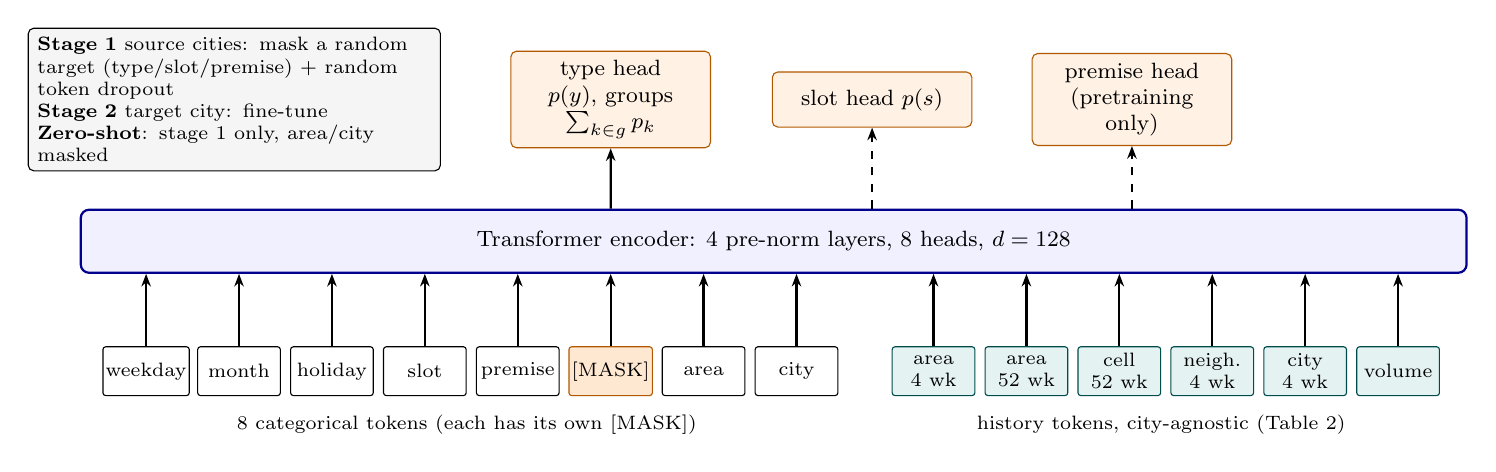
\begin{tikzpicture}[font=\footnotesize,
  tok/.style={draw, rounded corners=1pt, minimum width=1.05cm, minimum height=0.62cm, fill=white, align=center, inner sep=1pt, font=\scriptsize},
  msk/.style={tok, fill=orange!18, draw=orange!70!black},
  hst/.style={tok, fill=teal!10, draw=teal!60!black},
  blk/.style={draw, rounded corners=3pt, thick, fill=blue!6, draw=blue!55!black, minimum height=0.8cm, align=center},
  hd/.style={draw, rounded corners=2pt, fill=orange!10, draw=orange!70!black, align=center, minimum height=0.7cm, text width=2.3cm},
  arr/.style={-{Stealth[length=1.6mm]}, thick}]
\foreach \l [count=\i] in {weekday, month, holiday, slot, premise, {[MASK]}, area, city}{
  \ifnum\i=6 \node[msk] (c\i) at (\i*1.18,0) {\l}; \else \node[tok] (c\i) at (\i*1.18,0) {\l}; \fi}
\foreach \l [count=\i] in {area\\4 wk, area\\52 wk, cell\\52 wk, neigh.\\4 wk, city\\4 wk, volume}{
  \node[hst] (h\i) at (10.0+\i*1.18,0) {\l};}
\node[font=\scriptsize, below=0.12cm of c4.south east] {8 categorical tokens (each has its own [MASK])};
\node[font=\scriptsize, below=0.12cm of h3.south east] {history tokens, city-agnostic (Table 2)};
\node[blk, minimum width=17.6cm] (enc) at (9.15,1.65) {Transformer encoder: 4 pre-norm layers, 8 heads, $d=128$};
\foreach \i in {1,...,8} \draw[arr] (c\i.north) -- (c\i.north |- enc.south);
\foreach \i in {1,...,6} \draw[arr] (h\i.north) -- (h\i.north |- enc.south);
\node[hd] (ht) at (7.08,3.45) {type head\\$p(y)$, groups $\sum_{k\in g}p_k$};
\node[hd] (hs) at (10.4,3.45) {slot head $p(s)$};
\node[hd] (hp) at (13.7,3.45) {premise head\\(pretraining only)};
\draw[arr] (c6.north |- enc.north) -- (ht.south);
\draw[arr, dashed] (enc.north -| hs.south) -- (hs.south);
\draw[arr, dashed] (enc.north -| hp.south) -- (hp.south);
\node[draw, rounded corners=2pt, fill=gray!8, align=left, text width=5.0cm, font=\scriptsize] at (2.3,3.45)
 {\textbf{Stage 1} source cities: mask a random target (type/slot/premise) + random token dropout\\
  \textbf{Stage 2} target city: fine-tune\\
  \textbf{Zero-shot}: stage 1 only, area/city masked};
\end{tikzpicture}}
\caption{\HMX{}. An incident is a set of tokens. The attribute to be predicted (here the crime type) is replaced by [MASK], and its contextualised representation feeds the attribute's head. The history boxes follow the rows of Table~\ref{tab:features}; the two area boxes and the city box each stand for two tokens (type mix and time-of-day mix), giving nine history tokens}
\label{fig:model}
\end{figure}

\subsection{Pretraining on source cities}
For a target city, the other two cities are the sources. Up to 1.2 million source incidents, split evenly between the sources, are used for four epochs. For each incident, one target attribute is drawn: crime type with probability 0.45, time slot 0.35 and premise 0.20 (only where the attribute is recorded). Its token is masked and the model predicts it. In addition, every other categorical token is dropped (replaced by [MASK]) with probability 0.10, area and city tokens with probability 0.30, and every history token with probability 0.05. Token dropout teaches the model to work without area identity, which zero-shot prediction requires, and with fields that a city does not record, such as San Francisco's premise. Because the masked attribute is always observed, the objective is multi-target supervised pretraining rather than reconstruction.

\subsection{Coherent hierarchy loss}
Let $p\in\Delta^{10}$ be the predicted type distribution, $g(k)$ the group of type $k$ and $\mathcal{S}(k)$ its siblings. The type loss is
\begin{equation}
\mathcal{L}_{\text{type}} = -\sum_{k} q_k \log p_k \;-\; \lambda \log \sum_{j:\,g(j)=g(y)} p_j,
\qquad q_k = (1-\epsilon)\,\mathbb{1}[k=y] + \frac{\epsilon}{|\mathcal{S}(y)|}\,\mathbb{1}[k\in\mathcal{S}(y)],
\label{eq:hier}
\end{equation}
with $\epsilon=0.05$ and $\lambda=0.3$. The first term is label smoothing \citep{szegedy2016} restricted to siblings. The second term is the cross-entropy of the group probability obtained by summing type probabilities, so predicted groups and types can never disagree. The slot and premise heads use plain cross-entropy.

\subsection{Fine-tuning and zero-shot use}
Fine-tuning on the target city continues the masked objective with task probabilities 0.5 (type), 0.4 (slot) and 0.1 (premise), lower token dropout (0.05 for area and city), and a learning rate of $3\times10^{-4}$. Early stopping uses the sum of validation log-losses for both tasks. \HMX{}-scratch is the same model trained on the target city only (learning rate $10^{-3}$). For zero-shot prediction (\HMX{}-zero), the pretrained model is applied without fine-tuning. Area and city tokens are masked, as is the premise wherever the target city does not record it, and the temperature is fitted on source validation data.

\subsection{Training details and use of generative AI}
All neural models use AdamW \citep{loshchilov2019} with weight decay $10^{-5}$, 3\% warm-up followed by cosine decay to 10\% of the peak rate, gradient clipping at 1, mixed precision, and early stopping with patience 5 on validation log-loss. The batch size is 256 to 2,048 depending on the training-set size. The number of epochs is $\min\!\big(60, \max(15, \mathrm{round}(2.5\times10^{6}/n))\big)$ for $n$ training incidents, which keeps the number of gradient updates comparable across budgets. Models were implemented in PyTorch \citep{paszke2019} and trained on one NVIDIA T4 GPU. \emph{Use of generative AI.} An AI assistant (Claude, Anthropic) was used to help design and implement the experiment code and the analysis scripts and to draft parts of the manuscript text. The authors ran all experiments, checked all code, numbers and text, and take full responsibility for the content.

% ======================================================================
\section{Experimental design}\label{sec:design}

\subsection{Baselines}
All learned models receive the same inputs: the six categorical attributes other than the target, area included, and the 73 history features. They are as follows.
\begin{itemize}
\item \textbf{Target-only models.} Prior (smoothed class frequencies); \emph{Hist}, the average of the area's four-week and the cell's 52-week mix; multinomial logistic regression (LogReg); \textbf{GBDT}, XGBoost \citep{chen2016xgboost} with native categorical splits, learning rate 0.08, depth 7 and early stopping after 50 rounds; a multilayer perceptron with entity embeddings (MLP, three layers of 256 units); \textbf{TabM-mini} \citep{gorishniy2025}, with 32 ensemble members sharing one MLP through multiplicative input adapters; the \textbf{FT-Transformer} (FTT; three layers, $d=96$) \citep{gorishniy2021}; \textbf{TabICL} \citep{qu2025tabicl}, version-2 checkpoint \citep{qu2026tabiclv2}, with up to 10,000 in-context training rows, run for budgets up to 52 weeks and three seeds; and \HMX{}-scratch.
\item \textbf{Transfer models.} \textbf{GBDT-pool}, XGBoost trained on 200,000 source incidents plus the target incidents, with target rows up-weighted so that their total weight is at least half that of the source rows; \textbf{FTT-pre}, an FT-Transformer pretrained for the same task on the same source incidents as \HMX{} and then fine-tuned, i.e. a strong, task-specific version of supervised pretraining \citep{levin2023}; \textbf{\HMX{}} (pretrained); and \HMX{}-zero.
\end{itemize}
No model was tuned on the test data. Hyperparameters were fixed before the experiments, using common defaults from the original papers.

\subsection{Protocol}
Each target city is combined with each budget, five seeds (0--4) and each model. FT-Transformer models use three seeds at the 52-week and full budgets, to save computing time. Every probabilistic model is temperature-scaled on the target validation weeks \citep{guo2017} before testing, so log-loss differences are not merely differences in calibration. The study comprises 1,464 main runs and 162 ablation runs. As a robustness check added after the main experiments, the whole time grid was then moved 26 weeks earlier, giving a second test window from 16 June to 14 December 2025, in the opposite season to the first. All data after this window were removed, target histories end at its start, and source pretraining uses only earlier weeks. This check covers budgets of 0, 4, 8 and 16 weeks, three seeds and all models except the MLP, which was never the best target-only model at these budgets in the main window, and adds 540 runs. Code, features and hyperparameters are unchanged.

\subsection{Metrics}
The primary metric is test log-loss (nats per incident), a proper scoring rule. Secondary metrics are macro-F1, rare-type F1 (mean F1 of the three least frequent types in the target training data), top-3 accuracy, expected calibration error (ECE; 15 bins) and the \emph{expected mistake severity} $\mathbb{E}_{k\sim p}[d(y,k)]$. For types, $d$ is the distance in the two-level taxonomy (0, 1 for a sibling, 2 otherwise). For slots, it is the circular distance in four-hour steps.

\subsection{Statistical inference}
Incidents in the same week share shocks, so incidents are not independent observations. We therefore use a paired week-block bootstrap \citep{kunsch1989}: the 26 test weeks are resampled with replacement 2,000 times, every model is evaluated on the same resampled weeks, and seed results are averaged inside each replicate. A difference is called significant when its 95\% percentile interval excludes zero. For comparisons against the \emph{best target-only model}, that model is chosen per cell by mean test log-loss, which favours the baseline.

To test whether the benefit of transfer is spatially structured, we compute for every area with at least 20 test incidents the gain of a pretrained model over GBDT (GBDT log-loss minus the pretrained model's log-loss, averaged over seeds) and measure its global spatial autocorrelation with Moran's $I$ \citep{moran1950}. Areas are joined to the official boundaries of Chicago's community areas, New York's police precincts and San Francisco's analysis neighbourhoods \citep{chicagoca2026,nypdpct2026,sfnhood2026}; every area matched a polygon. We use row-standardised queen contiguity weights (polygons sharing a boundary point, with a 1~m tolerance) and, as a robustness check, five-nearest-neighbour weights on area centroids. Significance is assessed with 9,999 random permutations (two-sided). Because area volume is itself spatially clustered, we also compute $I$ for the residuals of a regression of the gain on the logarithm of the area's test volume, which asks whether gains cluster in space beyond what volume explains. These tests were added after the main experiments and are exploratory.

\subsection{Pre-specified hypotheses and protocol amendments}
Seven hypotheses were written into the analysis code before any real-data run, with their decision rules. H1: with $\le$16 weeks, pretrained \HMX{} beats the best target-only model in $\ge$7 of 9 city--budget cells (O1). H2: it beats the best transfer baseline in $\ge$6 of 9 cells. H3: with full history, it is within 0.002 nats of the best model in all cities. H4: H1 for O2, in $\ge$6 of 9 cells. H5: the hierarchy loss lowers mistake severity without raising log-loss by more than 0.002. H6: zero-shot prediction beats the best four-week target-only model in $\ge$2 of 3 cities. H7: gains over GBDT at 8 weeks are larger in the lowest-volume fifth of areas than in the highest-volume fifth in $\ge$2 of 3 cities.

The protocol was amended twice, and both amendments are reported for transparency. (i) After the first city had been run, training logs showed that all neural models stopped at the epoch cap at the 52-week and full budgets. The minimum number of epochs was therefore raised to 15 for all neural models, and the affected Chicago runs were repeated. (ii) The specification stated that attributes a city does not record are masked, but the code masked San Francisco's premise only during fine-tuning, not in zero-shot use. After this was corrected, all zero-shot runs were repeated. Fine-tuned runs were unaffected, because they learn the meaning of the unknown premise from target data. Neither amendment used test results.

% ======================================================================
\section{Results}\label{sec:results}

\subsection{Overview}
Tables~\ref{tab:lltype} and~\ref{tab:llslot} report mean test log-loss and Fig.~\ref{fig:curves} the learning curves. Place and context carry substantial information about crime type. Relative to the class prior, the best model in each cell reduces log-loss by 0.17 to 0.30 nats, and top-3 accuracy at eight weeks is 0.71 to 0.80 (Online Resource 1). Time of day is harder to predict, with improvements over the prior of 0.03 to 0.07 nats. The standard deviation of log-loss across seeds has a median of 0.0022 for O1 and 0.0011 for O2, so differences of a few thousandths of a nat can be reliable, which the paired bootstrap tests directly.

\begin{table}[!htbp]
\centering
\caption{O1 crime type: test log-loss after temperature scaling, mean over seeds (lower is better; bold = best in row). Weeks = target history. GBDT-pool, FTT-pre and HMX-pre use the two other cities as sources; HMX-scr is \HMX{} trained on the target city only. TabICL is not run on the full history. Standard deviations and the other baselines are given in Online Resource 1}
\label{tab:lltype}
\footnotesize
\setlength{\tabcolsep}{4pt}
\begin{tabular}{llcccccccc}
\toprule
 & & \multicolumn{5}{c}{Target only} & \multicolumn{3}{c}{With source cities} \\
\cmidrule(lr){3-7}\cmidrule(lr){8-10}
City & Weeks & GBDT & TabM-mini & FTT & TabICL & HMX-scr & GBDT-pool & FTT-pre & HMX-pre \\
\midrule
\multirow{6}{*}{Chicago} & 4 & 1.6966 & 1.6918 & 1.6742 & 1.6835 & 1.6857 & 1.7014 & \textbf{1.6501} & 1.6513 \\
 & 8 & 1.6631 & 1.6427 & 1.6528 & 1.6588 & 1.6608 & 1.6681 & \textbf{1.6338} & 1.6383 \\
 & 16 & 1.6403 & 1.6242 & 1.6398 & 1.6427 & 1.6490 & 1.6447 & \textbf{1.6233} & 1.6309 \\
 & 52 & 1.6224 & \textbf{1.6163} & 1.6221 & 1.6417 & 1.6213 & 1.6225 & 1.6171 & 1.6190 \\
 & all & 1.6239 & 1.6188 & 1.6181 & -- & 1.6183 & 1.6277 & \textbf{1.6132} & 1.6221 \\
 & 0 (zero-shot) & \multicolumn{8}{l}{HMX-zero: 1.7713 (prior at 4 weeks: 1.9009)} \\
\midrule
\multirow{6}{*}{New York} & 4 & 1.5207 & 1.5303 & 1.5226 & 1.5468 & 1.5455 & 1.5225 & \textbf{1.5070} & 1.5154 \\
 & 8 & 1.4920 & 1.4927 & 1.4949 & 1.5285 & 1.5187 & 1.4927 & \textbf{1.4883} & 1.4918 \\
 & 16 & 1.4692 & \textbf{1.4602} & 1.4751 & 1.4992 & 1.4836 & 1.4700 & 1.4670 & 1.4763 \\
 & 52 & 1.4462 & 1.4552 & 1.4544 & 1.4880 & 1.4599 & \textbf{1.4456} & 1.4542 & 1.4601 \\
 & all & 1.4520 & 1.4590 & 1.4553 & -- & 1.4630 & \textbf{1.4514} & 1.4567 & 1.4656 \\
 & 0 (zero-shot) & \multicolumn{8}{l}{HMX-zero: 1.6290 (prior at 4 weeks: 1.7422)} \\
\midrule
\multirow{6}{*}{San Francisco} & 4 & 1.8007 & 1.8373 & 1.7902 & 1.8385 & 1.8173 & 1.7925 & 1.7511 & \textbf{1.7508} \\
 & 8 & 1.7778 & 1.8107 & 1.7796 & 1.7608 & 1.7800 & 1.7669 & \textbf{1.7425} & 1.7428 \\
 & 16 & 1.7466 & \textbf{1.7260} & 1.7448 & 1.7362 & 1.7573 & 1.7388 & 1.7298 & 1.7293 \\
 & 52 & 1.7393 & \textbf{1.7163} & 1.7317 & 1.7408 & 1.7355 & 1.7259 & 1.7246 & 1.7256 \\
 & all & 1.7229 & \textbf{1.7133} & 1.7234 & -- & 1.7220 & 1.7187 & 1.7162 & 1.7177 \\
 & 0 (zero-shot) & \multicolumn{8}{l}{HMX-zero: 1.7765 (prior at 4 weeks: 1.9205)} \\

\bottomrule
\end{tabular}
\end{table}

\begin{table}[!htbp]
\centering
\caption{O2 time of day: test log-loss after temperature scaling, mean over seeds. Layout as in Table~\ref{tab:lltype}}
\label{tab:llslot}
\footnotesize
\setlength{\tabcolsep}{4pt}
\begin{tabular}{llcccccccc}
\toprule
 & & \multicolumn{5}{c}{Target only} & \multicolumn{3}{c}{With source cities} \\
\cmidrule(lr){3-7}\cmidrule(lr){8-10}
City & Weeks & GBDT & TabM-mini & FTT & TabICL & HMX-scr & GBDT-pool & FTT-pre & HMX-pre \\
\midrule
\multirow{6}{*}{Chicago} & 4 & 1.7316 & 1.7206 & 1.7161 & 1.7260 & 1.7158 & 1.7318 & \textbf{1.6980} & 1.7003 \\
 & 8 & 1.7151 & 1.7013 & 1.7076 & 1.7179 & 1.7148 & 1.7152 & 1.6956 & \textbf{1.6948} \\
 & 16 & 1.7049 & 1.6920 & 1.6964 & 1.7067 & 1.7005 & 1.7032 & \textbf{1.6901} & 1.6918 \\
 & 52 & 1.6919 & \textbf{1.6848} & 1.6888 & 1.6993 & 1.6862 & 1.6915 & 1.6859 & 1.6858 \\
 & all & 1.6902 & 1.6860 & 1.6872 & -- & 1.6868 & 1.6897 & \textbf{1.6859} & 1.6873 \\
 & 0 (zero-shot) & \multicolumn{8}{l}{HMX-zero: 1.7076 (prior at 4 weeks: 1.7550)} \\
\midrule
\multirow{6}{*}{New York} & 4 & 1.6888 & 1.6794 & 1.6816 & 1.6997 & 1.6881 & 1.6880 & \textbf{1.6708} & 1.6747 \\
 & 8 & 1.6782 & 1.6716 & 1.6725 & 1.6952 & 1.6760 & 1.6778 & \textbf{1.6670} & 1.6683 \\
 & 16 & 1.6685 & \textbf{1.6587} & 1.6655 & 1.6845 & 1.6660 & 1.6688 & 1.6623 & 1.6617 \\
 & 52 & 1.6573 & \textbf{1.6551} & 1.6595 & 1.6736 & 1.6564 & 1.6581 & 1.6572 & 1.6568 \\
 & all & 1.6613 & 1.6588 & 1.6599 & -- & 1.6599 & 1.6617 & \textbf{1.6582} & 1.6606 \\
 & 0 (zero-shot) & \multicolumn{8}{l}{HMX-zero: 1.6935 (prior at 4 weeks: 1.7241)} \\
\midrule
\multirow{6}{*}{San Francisco} & 4 & 1.7179 & 1.7111 & 1.7341 & 1.7079 & 1.7243 & 1.7229 & 1.6996 & \textbf{1.6992} \\
 & 8 & 1.7113 & 1.7085 & 1.7152 & 1.7061 & 1.7160 & 1.7155 & \textbf{1.6961} & 1.6991 \\
 & 16 & 1.7035 & 1.6931 & 1.6993 & 1.6940 & 1.7053 & 1.7039 & \textbf{1.6905} & 1.6944 \\
 & 52 & 1.6945 & \textbf{1.6855} & 1.6990 & 1.6932 & 1.6973 & 1.6938 & 1.6903 & 1.6925 \\
 & all & 1.6894 & \textbf{1.6854} & 1.6888 & -- & 1.6873 & 1.6879 & 1.6865 & 1.6894 \\
 & 0 (zero-shot) & \multicolumn{8}{l}{HMX-zero: 1.7082 (prior at 4 weeks: 1.7288)} \\

\bottomrule
\end{tabular}
\end{table}

\begin{figure}[!htbp]
\centering
\includegraphics[width=\textwidth]{figures/Fig2.pdf}
\caption{Learning curves in the main test window. Test log-loss against weeks of target-city history for the two strongest target-only models and the two source-pretrained models; the dashed line is \HMX{} applied without any target training. Panels (a)--(c) crime type, (d)--(f) time of day}
\label{fig:curves}
\end{figure}

\subsection{When does pretraining help?}
Fig.~\ref{fig:gain} and Table~\ref{tab:paired} give paired differences between source-pretrained models and the best target-only model in each cell of the main test window. With four or eight weeks of history, FTT-pre improved on the best target-only model in all 12 city--task--budget cells, and \HMX{} in 11 of 12 (the exception, New York O1 at eight weeks, was a tie). For crime type with four weeks, the reduction in log-loss was 0.024 nats in Chicago (95\% interval 0.022--0.026), 0.014 in New York (0.011--0.016) and 0.028 in San Francisco (0.020--0.036). For time of day, it was 0.018, 0.009 and 0.009 nats. At eight weeks the gains roughly halved. In accuracy terms the effects are modest: across the 12 short-budget cells, FTT-pre changed top-1 accuracy relative to the best target-only model by $-0.1$ to $+1.5$ percentage points and top-3 accuracy by 0.0 to $+1.6$ points, because log-loss also rewards better-calibrated probabilities for the less likely classes. The data multipliers below give a more practical reading. By 16 weeks they had largely disappeared: FTT-pre was better in one, tied in two and worse in three of six cells, and with 52 weeks or the full history it was better in two, tied in four and worse in six of twelve.

The benefit is a property of pretraining rather than of a particular architecture. Pretraining improved \HMX{} over the same model trained from scratch in all 12 cells at four and eight weeks and in all six cells at 16 weeks, with crime-type gains of 0.034, 0.030 and 0.066 nats at four weeks in Chicago, New York and San Francisco. Interpolating the target-only learning curves of the main window, the best target-only model needs 1.1 to 3.0 times as many weeks of local data to reach the four-week log-loss of \HMX{}, with the largest factors in San Francisco (2.9 for crime type, 3.0 for time of day; Online Resource 1).

\begin{figure}[!htbp]
\centering
\includegraphics[width=\textwidth]{figures/Fig3.pdf}
\caption{Effect of source pretraining in the main test window. Difference in test log-loss between the source-pretrained FT-Transformer and the best target-only model of each cell, with 95\% week-block bootstrap intervals. Negative values mean that pretraining helps. (a) crime type, (b) time of day}
\label{fig:gain}
\end{figure}

\begin{table}[!htbp]
\centering
\caption{O1 crime type, main test window: paired differences in test log-loss, A $-$ B, with 95\% week-block bootstrap intervals. \textbf{Bold}: A significantly better; \textit{italic}: A significantly worse. "Best target-only" is the target-only model with the lowest mean log-loss in that row (named in column 3). CHI Chicago, NYC New York, SF San Francisco. Results for O2 are in Online Resource 1}
\label{tab:paired}
\scriptsize
\setlength{\tabcolsep}{2.5pt}
\begin{tabular}{lllcccc}
\toprule
City & Wk & Best target-only & FTT-pre $-$ best & HMX-pre $-$ best & HMX-pre $-$ FTT-pre & GBDT-pool $-$ GBDT \\
\midrule
\multirow{5}{*}{CHI} & 4 & FTT & \textbf{$-$0.024 [$-$0.026, $-$0.022]} & \textbf{$-$0.023 [$-$0.025, $-$0.021]} & $+$0.001 [0.000, $+$0.002] & \textit{$+$0.005 [$+$0.003, $+$0.007]} \\
 & 8 & TabM-mini & \textbf{$-$0.009 [$-$0.013, $-$0.005]} & \textbf{$-$0.004 [$-$0.008, $-$0.001]} & \textit{$+$0.005 [$+$0.003, $+$0.006]} & \textit{$+$0.005 [$+$0.004, $+$0.007]} \\
 & 16 & TabM-mini & $-$0.001 [$-$0.003, $+$0.001] & \textit{$+$0.007 [$+$0.005, $+$0.008]} & \textit{$+$0.008 [$+$0.006, $+$0.009]} & \textit{$+$0.004 [$+$0.003, $+$0.005]} \\
 & 52 & TabM-mini & $+$0.001 [0.000, $+$0.003] & \textit{$+$0.003 [$+$0.001, $+$0.004]} & \textit{$+$0.002 [$+$0.001, $+$0.004]} & 0.000 [$-$0.001, $+$0.001] \\
 & all & MLP & \textbf{$-$0.004 [$-$0.006, $-$0.002]} & \textit{$+$0.006 [$+$0.004, $+$0.009]} & \textit{$+$0.009 [$+$0.007, $+$0.011]} & \textit{$+$0.004 [$+$0.003, $+$0.005]} \\
\midrule
\multirow{5}{*}{NYC} & 4 & GBDT & \textbf{$-$0.014 [$-$0.016, $-$0.011]} & \textbf{$-$0.005 [$-$0.009, $-$0.002]} & \textit{$+$0.008 [$+$0.006, $+$0.011]} & \textit{$+$0.002 [0.000, $+$0.004]} \\
 & 8 & GBDT & \textbf{$-$0.004 [$-$0.006, $-$0.002]} & 0.000 [$-$0.002, $+$0.002] & \textit{$+$0.004 [$+$0.002, $+$0.005]} & $+$0.001 [$-$0.001, $+$0.002] \\
 & 16 & TabM-mini & \textit{$+$0.007 [$+$0.006, $+$0.008]} & \textit{$+$0.016 [$+$0.015, $+$0.017]} & \textit{$+$0.009 [$+$0.009, $+$0.010]} & $+$0.001 [0.000, $+$0.002] \\
 & 52 & GBDT & \textit{$+$0.008 [$+$0.007, $+$0.009]} & \textit{$+$0.014 [$+$0.012, $+$0.016]} & \textit{$+$0.006 [$+$0.005, $+$0.008]} & \textbf{$-$0.001 [$-$0.001, 0.000]} \\
 & all & GBDT & \textit{$+$0.004 [$+$0.003, $+$0.006]} & \textit{$+$0.014 [$+$0.012, $+$0.015]} & \textit{$+$0.009 [$+$0.008, $+$0.010]} & $-$0.001 [$-$0.001, 0.000] \\
\midrule
\multirow{5}{*}{SF} & 4 & Hist & \textbf{$-$0.028 [$-$0.036, $-$0.020]} & \textbf{$-$0.028 [$-$0.037, $-$0.021]} & 0.000 [$-$0.003, $+$0.002] & \textbf{$-$0.008 [$-$0.011, $-$0.005]} \\
 & 8 & TabICL & \textbf{$-$0.015 [$-$0.022, $-$0.008]} & \textbf{$-$0.018 [$-$0.027, $-$0.011]} & 0.000 [$-$0.002, $+$0.002] & \textbf{$-$0.011 [$-$0.014, $-$0.008]} \\
 & 16 & TabM-mini & \textit{$+$0.004 [$+$0.002, $+$0.006]} & $+$0.003 [0.000, $+$0.007] & $-$0.001 [$-$0.004, $+$0.003] & \textbf{$-$0.008 [$-$0.011, $-$0.005]} \\
 & 52 & TabM-mini & \textit{$+$0.009 [$+$0.006, $+$0.012]} & \textit{$+$0.009 [$+$0.006, $+$0.012]} & $+$0.003 [$-$0.002, $+$0.007] & \textbf{$-$0.013 [$-$0.017, $-$0.010]} \\
 & all & TabM-mini & $+$0.003 [$-$0.001, $+$0.007] & \textit{$+$0.004 [$+$0.001, $+$0.008]} & $+$0.001 [$-$0.002, $+$0.005] & \textbf{$-$0.004 [$-$0.007, $-$0.002]} \\

\bottomrule
\end{tabular}
\end{table}

\subsection{A second test window}\label{sec:window2}
Table~\ref{tab:window2} repeats the comparison on the second test window (June to December 2025). The four-week result replicated. FTT-pre beat the best target-only model in five of six cells and tied in the sixth (San Francisco, time of day), and \HMX{} beat it in all six, with crime-type gains of 0.027, 0.012 and 0.035 nats (FTT-pre) in Chicago, New York and San Francisco. At eight weeks the benefit was weaker than in the first window: FTT-pre was better in two cells and tied in four, and \HMX{} was better in three, tied in two and worse in one. San Francisco, the smallest city, still gained 0.027 nats for crime type. At 16 weeks neither pretrained model was better in any cell. Over both windows, source pretraining thus improved on the best local model in 23 of 24 four-week cells, in 16 of 24 eight-week cells, and in one of 24 sixteen-week cells. The time scale of the benefit is therefore robust, but its tail depends on the season: in the summer-to-autumn window, a clear eight-week benefit remained only in San Francisco, with a small one (about 0.002 nats) for time of day in Chicago. The other findings also replicated: pretraining improved \HMX{} over training from scratch in all 18 cells, \HMX{} beat FTT-pre in only two of 18 cells, and zero-shot prediction beat four weeks of local data for time of day in Chicago, as in the main window, and now also in San Francisco, but again not for crime type in the two large cities (Online Resource 1).

\begin{table}[!htbp]
\centering
\caption{Robustness to the test window. Difference in test log-loss between each source-pretrained model and the best target-only model of the cell (negative = pretraining helps) in the main window (15 December 2025 -- 14 June 2026; five seeds) and in a second window 26 weeks earlier (16 June -- 14 December 2025; three seeds). \textbf{Bold}: significantly better; \textit{italic}: significantly worse (95\% week-block bootstrap). Intervals are given in Online Resource 1}
\label{tab:window2}
\footnotesize
\setlength{\tabcolsep}{4pt}
\begin{tabular}{lllcccccc}
\toprule
 & & & \multicolumn{3}{c}{Window 1: weeks of history} & \multicolumn{3}{c}{Window 2: weeks of history} \\
\cmidrule(lr){4-6}\cmidrule(lr){7-9}
Task & City & Model & 4 & 8 & 16 & 4 & 8 & 16 \\
\midrule
\multirow{6}{*}{O1 type} & \multirow{2}{*}{Chicago} & FTT-pre & \textbf{$-$0.024} & \textbf{$-$0.009} & $-$0.001 & \textbf{$-$0.027} & $+$0.002 & \textit{$+$0.006} \\
 &  & HMX-pre & \textbf{$-$0.023} & \textbf{$-$0.004} & \textit{$+$0.007} & \textbf{$-$0.026} & $+$0.002 & \textit{$+$0.007} \\
\cmidrule(lr){2-9}
 & \multirow{2}{*}{New York} & FTT-pre & \textbf{$-$0.014} & \textbf{$-$0.004} & \textit{$+$0.007} & \textbf{$-$0.012} & $-$0.002 & \textit{$+$0.004} \\
 &  & HMX-pre & \textbf{$-$0.005} & 0.000 & \textit{$+$0.016} & \textbf{$-$0.007} & \textit{$+$0.008} & \textit{$+$0.011} \\
\cmidrule(lr){2-9}
 & \multirow{2}{*}{San Francisco} & FTT-pre & \textbf{$-$0.028} & \textbf{$-$0.015} & \textit{$+$0.004} & \textbf{$-$0.035} & \textbf{$-$0.027} & $-$0.003 \\
 &  & HMX-pre & \textbf{$-$0.028} & \textbf{$-$0.018} & $+$0.003 & \textbf{$-$0.037} & \textbf{$-$0.032} & $-$0.002 \\
\midrule
\multirow{6}{*}{O2 time} & \multirow{2}{*}{Chicago} & FTT-pre & \textbf{$-$0.018} & \textbf{$-$0.006} & \textbf{$-$0.002} & \textbf{$-$0.011} & \textbf{$-$0.002} & \textit{$+$0.001} \\
 &  & HMX-pre & \textbf{$-$0.016} & \textbf{$-$0.006} & 0.000 & \textbf{$-$0.009} & \textbf{$-$0.002} & \textit{$+$0.002} \\
\cmidrule(lr){2-9}
 & \multirow{2}{*}{New York} & FTT-pre & \textbf{$-$0.009} & \textbf{$-$0.005} & \textit{$+$0.004} & \textbf{$-$0.009} & $-$0.001 & \textit{$+$0.004} \\
 &  & HMX-pre & \textbf{$-$0.005} & \textbf{$-$0.003} & \textit{$+$0.003} & \textbf{$-$0.007} & 0.000 & \textit{$+$0.003} \\
\cmidrule(lr){2-9}
 & \multirow{2}{*}{San Francisco} & FTT-pre & \textbf{$-$0.009} & \textbf{$-$0.009} & $-$0.003 & $-$0.001 & $-$0.004 & $-$0.002 \\
 &  & HMX-pre & \textbf{$-$0.010} & \textbf{$-$0.010} & $+$0.001 & \textbf{$-$0.005} & \textbf{$-$0.004} & 0.000 \\

\bottomrule
\end{tabular}
\end{table}

\subsection{Pooling raw incidents is not a substitute}
Adding source incidents directly to the GBDT training set helped only in the smallest city. For crime type, GBDT-pool improved on GBDT in San Francisco at every budget, by 0.004 to 0.013 nats, but was worse in Chicago at four, eight and 16 weeks and on the full history, and mostly tied in New York (Table~\ref{tab:paired}). Over the twelve cells with four or eight weeks it was better in two, tied in five and worse in five. In the second window the picture was again mixed: for crime type, pooling helped only in San Francisco and hurt in Chicago, whereas for time of day it gave small gains of about 0.0015 nats in the two large cities. Pooled rows carry the source cities' label distributions, and a tree ensemble cannot separate structure that transfers from city-specific base rates. Pretrained representations, fine-tuned on the target, can.

\subsection{\HMX{} versus a task-specific pretrained transformer}
In the main window \HMX{} never beat FTT-pre significantly. Over all 30 cells it tied in 12 and was worse in 18, by 0.001 to 0.009 nats (Table~\ref{tab:paired}). The difference vanished in San Francisco, where the two were indistinguishable for crime type at every short budget. \HMX{} offers three practical advantages. One model serves both tasks and all three heads. Its training is faster: excluding pretraining, one run for both tasks took 24~s against 112~s for the two FT-Transformers at eight weeks (4.8 times faster) and 274~s against 2,537~s on the full history (9.3 times). And it can be used before any target data exist. The ablations (Section~\ref{sec:ablation}) show that part of the gap is the price of the hierarchy loss. Against the target-only models, \HMX{} trailed with 52 weeks or more, where all neural models ran into the fixed epoch budget (Section~\ref{sec:limitations}).

\subsection{Zero-shot prediction}
Without any target training data, \HMX{}-zero improved on the class prior in every case (Tables~\ref{tab:lltype} and~\ref{tab:llslot}). In the main window it matched the best four-week target-only model for crime type in San Francisco (difference $-$0.0027, interval $-$0.0139 to $+$0.0120) and for time of day in San Francisco ($+$0.0003, $-$0.0033 to $+$0.0039), and it beat it for time of day in Chicago ($-$0.0083, $-$0.0103 to $-$0.0063). In the other three cases, Chicago and New York crime type and New York time of day, four weeks of local data were better, by 0.097, 0.108 and 0.014 nats. Zero-shot prediction is therefore most useful where label distributions transfer, as for time of day, or where local data are scarce, as in San Francisco.

\subsection{Calibration, rare types and mistake severity}
Table~\ref{tab:secondary} reports secondary metrics at eight weeks. The pretrained models had the highest macro-F1 in every city: FTT-pre in Chicago and New York (0.206 and 0.194) and \HMX{} in San Francisco (0.139, against 0.130 for GBDT). Rare-type F1 benefited most from pretraining in Chicago, where FTT-pre reached 0.114 against 0.101 for GBDT. Both pretrained models were well calibrated after temperature scaling (ECE at most 0.038). Expected mistake severity has to be read together with log-loss: models that rarely predict outside the most frequent group, such as TabM-mini and the MLP at short budgets, obtain low severity despite poor log-loss and, for TabM-mini in San Francisco, poor calibration (ECE 0.132). Among the two competitive pretrained models, \HMX{} had a lower severity than FTT-pre in Chicago and New York (1.223 vs 1.237 and 1.133 vs 1.149) and a similar one in San Francisco. The controlled comparison in the ablations (Section~\ref{sec:ablation}) isolates the effect of the hierarchy loss.

\begin{table}[!htbp]
\centering
\caption{O1 crime type, eight weeks of target history: macro-F1 (mF1), rare-type F1 (rF1), expected mistake severity (E[sev], lower is better) and expected calibration error (ECE, lower is better). Means over seeds}
\label{tab:secondary}
\footnotesize
\setlength{\tabcolsep}{3pt}
\begin{tabular}{lcccccccccccc}
\toprule
 & \multicolumn{2}{c}{Chicago} & \multicolumn{2}{c}{New York} & \multicolumn{2}{c}{San Francisco} & \multicolumn{3}{c}{E[sev]} & \multicolumn{3}{c}{ECE} \\
\cmidrule(lr){2-3}\cmidrule(lr){4-5}\cmidrule(lr){6-7}\cmidrule(lr){8-10}\cmidrule(lr){11-13}
Model & mF1 & rF1 & mF1 & rF1 & mF1 & rF1 & CHI & NYC & SF & CHI & NYC & SF \\
\midrule
GBDT & 0.191 & 0.101 & 0.189 & 0.147 & 0.130 & 0.160 & 1.246 & 1.146 & 1.233 & 0.018 & 0.013 & 0.037 \\
TabM-mini & 0.179 & 0.054 & 0.152 & 0.112 & 0.093 & 0.118 & 1.228 & 1.130 & 1.194 & 0.019 & 0.040 & 0.132 \\
FTT & 0.197 & 0.085 & 0.181 & 0.134 & 0.118 & 0.163 & 1.242 & 1.148 & 1.224 & 0.015 & 0.009 & 0.056 \\
TabICL & 0.153 & 0.015 & 0.137 & 0.112 & 0.094 & 0.130 & 1.260 & 1.175 & 1.236 & 0.012 & 0.034 & 0.047 \\
GBDT-pool & 0.188 & 0.106 & 0.186 & 0.138 & 0.132 & 0.164 & 1.253 & 1.149 & 1.238 & 0.014 & 0.011 & 0.025 \\
FTT-pre & 0.206 & 0.114 & 0.194 & 0.149 & 0.122 & 0.164 & 1.237 & 1.149 & 1.219 & 0.010 & 0.009 & 0.038 \\
HMX-scr & 0.192 & 0.074 & 0.178 & 0.134 & 0.112 & 0.137 & 1.239 & 1.143 & 1.231 & 0.016 & 0.014 & 0.043 \\
HMX-pre & 0.205 & 0.101 & 0.193 & 0.140 & 0.139 & 0.164 & 1.223 & 1.133 & 1.222 & 0.014 & 0.013 & 0.034 \\

\bottomrule
\end{tabular}
\end{table}

\subsection{Where does transfer help?}
Fig.~\ref{fig:area} compares \HMX{} with GBDT area by area at eight weeks. In all three cities, gains were largest in low-volume areas. The Spearman correlation between an area's number of test incidents and the gain was $-0.29$ in Chicago, $-0.21$ in New York and $-0.56$ in San Francisco, and H7 was supported in all three. \HMX{} improved on GBDT in 96\% of Chicago's community areas and 89\% of San Francisco's neighbourhoods, but in only 47\% of New York's precincts, plausibly because large precinct volumes leave less room for borrowed structure. This pattern is what one would expect if pretraining supplies a prior over how local crime mixes evolve, which matters most where the local signal is weakest.

\begin{figure}[!htbp]
\centering
\includegraphics[width=\textwidth]{figures/Fig4.pdf}
\caption{Area-level gains at eight weeks of history. Each point is one area with at least 20 test incidents. Vertical axis: GBDT log-loss minus \HMX{} log-loss (crime type), averaged over five seeds. (a) Chicago community areas, (b) New York precincts, (c) San Francisco analysis neighbourhoods}
\label{fig:area}
\end{figure}

Fig.~\ref{fig:maps} maps the same gains and Table~\ref{tab:moran} tests whether they cluster in space. With contiguity weights, the gains were positively autocorrelated in San Francisco ($I = 0.18$, $p = 0.04$) but not in Chicago or New York; with nearest-neighbour weights, they were also clustered in Chicago ($I = 0.14$, $p = 0.02$). In every city and with both weightings, this structure disappeared once area volume was accounted for: Moran's $I$ of the residual gain was between $-0.03$ and $0.08$, with no $p$ below 0.14. The same held in all robustness checks (four weeks of history, FT-Transformer instead of \HMX{}, time of day, and 52 weeks): raw gains were clustered in 10 of 30 tests, but residual gains in none (smallest $p = 0.07$; Online Resource 1). Area volume itself was clustered where the gains were: Moran's $I$ of log test volume was 0.33 in Chicago ($p < 0.001$) and 0.28 in San Francisco ($p = 0.002$), but only 0.09 in New York ($p = 0.18$), where the gains showed no clustering either. Where transfer helps is therefore not a matter of particular neighbourhoods: the gain follows volume, and volume happens to be spatially clustered. For practice, this means that an agency can anticipate where a transferred model will help from local incident counts alone.

\begin{table}[!htbp]
\centering
\caption{Spatial autocorrelation of the area-level gain of \HMX{} over GBDT (crime type, eight weeks). Moran's $I$ with two-sided permutation $p$-values (9,999 permutations) in parentheses; bold: $p < 0.05$. ``After volume'': residuals of a regression of the gain on log test volume. Areas: areas with at least 20 test incidents. In San Francisco one island area has no contiguous neighbour and is omitted from the contiguity test}
\label{tab:moran}
\small
\begin{tabular}{lccccc}
\toprule
 & & \multicolumn{2}{c}{Queen contiguity} & \multicolumn{2}{c}{5 nearest neighbours} \\
\cmidrule(lr){3-4}\cmidrule(lr){5-6}
City & Areas & Gain & After volume & Gain & After volume \\
\midrule
Chicago & 77 & 0.059 (0.229) & 0.000 (0.836) & \textbf{0.141} (0.020) & 0.077 (0.140) \\
New York & 78 & 0.060 (0.239) & $-$0.001 (0.864) & 0.039 (0.296) & $-$0.001 (0.856) \\
San Francisco & 38 & \textbf{0.184} (0.038) & $-$0.026 (0.986) & \textbf{0.193} (0.016) & $-$0.007 (0.813) \\

\bottomrule
\end{tabular}
\end{table}

\begin{figure}[!htbp]
\centering
\includegraphics[width=\textwidth]{figures/Fig5.pdf}
\caption{Maps of the area-level gain of \HMX{} over GBDT for crime type at eight weeks (GBDT log-loss minus \HMX{} log-loss, mean over five seeds; blue: \HMX{} better). Moran's $I$ uses queen contiguity; ``after volume'' refers to residuals after regressing the gain on log test volume. Hatched: fewer than 20 test incidents. Boundaries: Chicago community areas, NYPD precincts, San Francisco analysis neighbourhoods. (a) Chicago, (b) New York, (c) San Francisco}
\label{fig:maps}
\end{figure}

\subsection{Ablations}\label{sec:ablation}
Each variant in Table~\ref{tab:ablation} and Fig.~\ref{fig:ablation} changes one component of \HMX{}. Pretraining and fine-tuning were repeated with three seeds at eight weeks, using 600,000 source incidents, and the variants are compared with a full model trained under the same settings.

\begin{itemize}
\item \textbf{History and context tokens matter most.} Removing the nine history tokens raised crime-type log-loss by 0.022 to 0.065 nats, and removing the cell, neighbour and city context by 0.011 to 0.048. This confirms that recent local crime mixes, the city-agnostic part of the input, carry the transferable signal.
\item \textbf{Multi-task pretraining helps.} Pretraining on crime type alone worsened time-of-day log-loss by 0.006 to 0.017 nats in all cities, and crime-type log-loss in New York and San Francisco.
\item \textbf{The hierarchy loss trades accuracy for better mistakes.} Removing it raised the expected mistake severity in all three cities, by 0.009 to 0.012, but lowered crime-type log-loss by 0.003 to 0.009. H5, which required no such cost, is therefore not supported. The hierarchy term is best seen as an adjustable knob, as in related work \citep{bertinetto2020}.
\item \textbf{Area and city identity add little} at eight weeks, which supports the design choice to rely on city-agnostic features. Token dropout helped slightly in Chicago and New York.
\item \textbf{Source selection matters.} Pretraining on San Francisco alone, the smallest city, was clearly worse for Chicago and New York, by 0.016 and 0.005 nats. Conversely, New York did better with Chicago as its only source than with Chicago and San Francisco together (by 0.005 nats). Adding a small source city can therefore cause negative transfer.
\end{itemize}

\begin{table}[!htbp]
\centering
\caption{Ablations at eight weeks: variant minus full \HMX{} (three seeds; positive = the variant is worse). $^{*}$: 95\% week-block bootstrap interval excludes zero. For single-source variants, the target city's own column is empty}
\label{tab:ablation}
\scriptsize
\setlength{\tabcolsep}{2.5pt}
\resizebox{\textwidth}{!}{%
\begin{tabular}{lccccccccc}
\toprule
 & \multicolumn{3}{c}{O1 $\Delta$ log-loss} & \multicolumn{3}{c}{O1 $\Delta$ E[severity]} & \multicolumn{3}{c}{O2 $\Delta$ log-loss} \\
\cmidrule(lr){2-4}\cmidrule(lr){5-7}\cmidrule(lr){8-10}
Variant & CHI & NYC & SF & CHI & NYC & SF & CHI & NYC & SF \\
\midrule
Remove history tokens & $+$0.0221$^{*}$ & $+$0.0646$^{*}$ & $+$0.0373$^{*}$ & $+$0.0077$^{*}$ & $+$0.0211$^{*}$ & $+$0.0158$^{*}$ & $+$0.0009$^{*}$ & $+$0.0049$^{*}$ & $+$0.0035$^{*}$ \\
Remove cell, neighbour and city context & $+$0.0107$^{*}$ & $+$0.0480$^{*}$ & $+$0.0146$^{*}$ & $+$0.0055$^{*}$ & $+$0.0196$^{*}$ & $+$0.0155$^{*}$ & $-$0.0005$^{*}$ & $+$0.0021$^{*}$ & $+$0.0020$^{*}$ \\
Pretrain on crime type only & $-$0.0006 & $+$0.0045$^{*}$ & $+$0.0102$^{*}$ & $+$0.0009$^{*}$ & $-$0.0032$^{*}$ & $+$0.0038$^{*}$ & $+$0.0118$^{*}$ & $+$0.0058$^{*}$ & $+$0.0173$^{*}$ \\
Remove hierarchy loss ($\epsilon=\lambda=0$) & $-$0.0031$^{*}$ & $-$0.0094$^{*}$ & $-$0.0038$^{*}$ & $+$0.0111$^{*}$ & $+$0.0121$^{*}$ & $+$0.0090$^{*}$ & $+$0.0011$^{*}$ & $-$0.0006$^{*}$ & 0.0000 \\
Remove token dropout & $+$0.0031$^{*}$ & $+$0.0026$^{*}$ & $-$0.0001 & $+$0.0006 & $+$0.0018$^{*}$ & $+$0.0025$^{*}$ & $-$0.0003 & $+$0.0002 & $+$0.0009$^{*}$ \\
Remove area and city tokens & $-$0.0015$^{*}$ & $-$0.0015$^{*}$ & $+$0.0012$^{*}$ & $+$0.0037$^{*}$ & $+$0.0016$^{*}$ & 0.0000 & $-$0.0002 & 0.0000 & $+$0.0005$^{*}$ \\
Single source: Chicago & -- & $-$0.0049$^{*}$ & $+$0.0042$^{*}$ & -- & $+$0.0037$^{*}$ & $-$0.0009 & -- & $+$0.0008$^{*}$ & $+$0.0035$^{*}$ \\
Single source: New York & $-$0.0004 & -- & $-$0.0024 & 0.0000 & -- & $-$0.0028$^{*}$ & $-$0.0013$^{*}$ & -- & $+$0.0014$^{*}$ \\
Single source: San Francisco & $+$0.0165$^{*}$ & $+$0.0053$^{*}$ & -- & $+$0.0067$^{*}$ & $+$0.0004 & -- & $+$0.0043$^{*}$ & $+$0.0040$^{*}$ & -- \\

\bottomrule
\end{tabular}}
\end{table}

\begin{figure}[!htbp]
\centering
\includegraphics[width=\textwidth]{figures/Fig6.pdf}
\caption{Ablations of \HMX{} for crime type at eight weeks, with 95\% week-block bootstrap intervals (three seeds). (a) Change in log-loss and (b) change in expected mistake severity, variant minus full model; positive values mean that the removed or changed component helped}
\label{fig:ablation}
\end{figure}

Masking single input tokens at test time leads to the same conclusion (Online Resource 1). For crime type, the premise token mattered most (log-loss rose by 0.095 when it was masked, averaged over cities at eight weeks), followed by the time slot (0.038) and the 52-week cell mix (0.033).

\subsection{Pre-specified hypotheses}
Table~\ref{tab:hyp} summarises the hypotheses. Two of seven were supported. The hypotheses refer to the main window; the second window was not part of the pre-specified plan. The central question has a clear answer: pretraining helps for the first one to two months of local history. The more ambitious claims for the specific architecture were not supported. H1 failed only because its decision rule included the 16-week cells, where no pretrained model was significantly better than the best target-only model for crime type.

\begin{table}[!htbp]
\centering
\caption{Pre-specified hypotheses and outcomes (decision rules as written before the experiments)}
\label{tab:hyp}
\scriptsize
\begin{tabular}{p{0.5cm}p{7.6cm}p{1.2cm}p{4.9cm}}
\toprule
 & Hypothesis & Cells passed & Outcome \\
\midrule
H1 & O1, $\le$16 weeks: \HMX{} beats best target-only model in $\ge$7 of 9 cells & 5 of 9 & Not supported (all 16-week cells fail; 5 of 6 short-budget cells pass) \\
H2 & O1, $\le$16 weeks: \HMX{} beats best transfer baseline in $\ge$6 of 9 cells & 0 of 9 & Not supported (FTT-pre stronger) \\
H3 & O1, full history: \HMX{} within 0.002 nats of best model in all cities & 0 of 3 & Not supported \\
H4 & O2, $\le$16 weeks: \HMX{} beats best target-only model in $\ge$6 of 9 cells & 6 of 9 & Supported \\
H5 & Hierarchy loss lowers severity at $\le$0.002 nats log-loss cost & 0 of 3 & Not supported (trade-off) \\
H6 & Zero-shot beats best 4-week target-only model in $\ge$2 of 3 cities & 1 of 3$^{a}$ & Not supported \\
H7 & Gains larger in lowest- than highest-volume fifth of areas in $\ge$2 of 3 cities & 3 of 3 & Supported \\
\bottomrule
\end{tabular}
\begin{flushleft}\footnotesize $^{a}$ By mean log-loss (San Francisco); with bootstrap intervals the San Francisco difference is a tie.\end{flushleft}
\end{table}

\FloatBarrier
% ======================================================================
\section{Discussion}\label{sec:discussion}

\subsection{Implications}
The main finding is a time scale. Where an agency or analyst has only a few weeks of comparable records, a model pretrained on other cities is consistently better than any model trained locally. This held in two test windows in opposite seasons. The advantage shrinks within one to two months, faster in some seasons than others, and is gone by about four months (16 weeks). Cross-city pretraining is therefore best understood as a bridge across a data gap, for example after a records-system migration, and not as a replacement for local data. The areas that benefit most are those with few incidents, where local estimates are noisiest. The spatial analysis sharpens this point: once volume is accounted for, the gains show no residual spatial clustering in any city, so we find no spatial clusters of neighbourhoods in which transfer helps or hurts more than their volume predicts. A simple operational rule follows, namely that a transferred model should be trusted most, and replaced last, in areas with few recorded incidents. Transfer is also most useful where it is most needed: for crime type, both the log-loss gain and the data multiplier were largest in the smallest city, San Francisco.

Two negative results are equally useful. First, simply concatenating records from other cities did not work reliably, because base rates differ between cities: theft is 25\% of harmonised incidents in Chicago but 46\% in San Francisco. Representations that are pretrained and then fine-tuned separate transferable structure from local base rates in a way that pooled tree ensembles cannot. Second, more sources are not automatically better. A small source city added noise for a larger target, which echoes findings on negative transfer in urban computing \citep{jin2022crosstres} and the finding of \citet{shan2026} that transfer performance depends on how the source and target cities differ. Our area-level results add a within-city counterpart: inside a target city, where transfer helps depends on local data volume rather than on location.

The design of \HMX{} suggests why transfer works at all. Its inputs describe recent local crime mixes in units that mean the same thing everywhere, and the ablations show that these inputs carry almost all of the signal, whereas area and city identity carry little. This is consistent with the criminology of place, in which crime concentrates at a small share of places and this concentration is stable over time \citep{weisburd2015}. It also suggests why transfer fades: once a city has a few months of its own history, the same features are estimated precisely from local data, and borrowed regularities add little.

\subsection{Responsible use}
Recorded crime is shaped by reporting and enforcement \citep{akpinar2021}, and models trained on it can entrench these patterns \citep{ensign2018}. Transfer adds a further risk: the source cities' recording practices are imported into the target. Our tasks concern incident attributes rather than the allocation of patrols, and we use no information about people. Even so, the area-level analysis shows that the benefits, and by implication the errors, are not evenly distributed. We recommend that any operational use be accompanied by area-level error audits and by monitoring of how a transferred model's predictions shift as local data accumulate.

\subsection{Limitations and threats to validity}\label{sec:limitations}
\emph{Scope.} Three large US cities, two test windows of 26 weeks (the second only for short histories) and two incident-level tasks do not establish generality. Cities with other legal taxonomies, or with smaller and rural agencies, may behave differently. \emph{Labels.} The keyword-based taxonomy necessarily merges categories that differ between jurisdictions. An audit of the released mapping (Online Resource 1, Table S23) also shows that ordered keyword rules misassign a few values. For premises, \textsc{warehouse} and \textsc{movie house} match the residential rule, \textsc{school yard} does too, \textsc{atm (automatic teller machine)} matches the vehicle rule, and \textsc{highway/parkway}, \textsc{pool room} and \textsc{bowling alley} fall into the park or street groups. For crime types, two New York descriptions truncated by the portal (\textsc{other offenses related to thef}, \textsc{unlawful poss.\ weap.\ on school}) are excluded, although their full forms would map to theft and weapons. Because every model receives the same labels and inputs, these errors do not favour any method, but they add noise to all of them. We release the mapping so that corrected or alternative mappings can be tested. \emph{Compute.} At the 52-week and full budgets, all neural models, including \HMX{}, reached the fixed maximum of 15 epochs, whereas GBDT used early stopping. The long-history comparison is therefore one at equal compute and probably understates the neural models. Our main conclusions concern the short budgets, where training converged. \emph{Seeds and coverage.} FT-Transformer models used three seeds at the long budgets, TabICL was limited to 10,000 in-context rows, and the ablations were run at one budget. \emph{Hyperparameters} were fixed and not tuned per model. Tuning could change the ranking of close competitors, but it would be unlikely to reverse effects of 0.01 to 0.03 nats. \emph{Seasonality and test windows.} With short budgets, the target city has not seen the months of the test window, whereas the source cities have, so part of the benefit may be seasonal knowledge. The second test window shows that the four-week benefit does not depend on the season but that the eight-week benefit does. Two windows are still a small sample of seasons, and the second window was run with three seeds and without the long budgets. \emph{Pre-registration.} The hypotheses were fixed in code before the experiments but were not registered with a third party.

% ======================================================================
\section{Conclusion}\label{sec:conclusion}

We built a benchmark to test whether knowledge transfers across cities for incident-level crime type and time prediction when local histories are short. Across Chicago, New York and San Francisco, models pretrained on other cities improved on all locally trained models with four weeks of history in two test windows in opposite seasons, and usually still at eight weeks, most of all in low-volume areas and, for crime type, in the smallest city. Their spatial pattern followed area volume, with no residual clustering. The advantage had disappeared by 16 weeks, about four months. Pooling raw records was not a substitute for pretraining, and a small source city could even harm a larger target. A masked multi-attribute transformer built on city-agnostic history features came close to a task-specific pretrained transformer, served both tasks with one model at a fraction of the training cost, and allowed useful predictions before any local data existed. Future work should extend the benchmark to more cities and other taxonomies, select source cities adaptively, and study how recording practices transfer along with predictive structure.

% ======================================================================
\section*{Statements and declarations}
\noindent\textbf{Funding} No funding was received for conducting this study.

\noindent\textbf{Competing interests} The authors have no relevant financial or non-financial interests to disclose.

\noindent\textbf{Data availability} All data are public: Chicago Data Portal datasets ijzp-q8t2 (incidents) and igwz-8jzy (community areas), NYC Open Data datasets qgea-i56i and 5uac-w243 (incidents) and y76i-bdw7 (police precincts), and DataSF datasets wg3w-h783 (incidents) and j2bu-swwd (analysis neighbourhoods), all accessed October 2026. The label mapping and all per-run results, including per-week and per-area statistics for every run, are provided in Online Resource 2 and in an anonymised repository for reviewers ([anonymised link]); the harmonised extracts are regenerated from the public portals by the released code. The repository will be deposited with a DOI on acceptance.

\noindent\textbf{Code availability} The complete pipeline (download, harmonisation, features, models, experiment runner and analysis) is available to reviewers in the same anonymised repository and will be released with a DOI on acceptance.

\noindent\textbf{Author contributions} Withheld for double-blind review; given on the title page.

\noindent\textbf{Ethics approval} Not applicable. The study uses only incident records that the agencies themselves publish without personal identifiers, and it uses only their offence, premise, time and area attributes.

\noindent\textbf{Online Resource 1} (ESM\_1.pdf) Full result tables (all models, mean $\pm$ s.d.), paired comparisons for O2, data multipliers, token-masking importance, the label mapping, all spatial autocorrelation tests and the full results of the second test window.

\noindent\textbf{Online Resource 2} (ESM\_2.zip) Machine-readable result tables (CSV) for both test windows: per-run metrics, paired bootstrap effects, ablations, spatial autocorrelation tests, area-level gains and the label mapping.

\bibliographystyle{plainnat}
\bibliography{references}

\end{document}
